\documentclass{article}

\usepackage{color}
\usepackage{graphicx}
\usepackage{tabularx}
\usepackage[frenchb]{babel}
\usepackage[utf8]{inputenc}
\usepackage[T1]{fontenc}
\usepackage{lmodern}


\usepackage{geometry}
 \geometry{
 top=25mm,
 bottom=25mm,
 }


\title{Document de présentation}
\author{Justal Kevin}
\date{26/09/2015}
\renewcommand{\contentsname}{Table des matières} 
 
\newcommand\invisiblesection[1]{%
  \refstepcounter{section}%
  \addcontentsline{toc}{section}{\protect\numberline{\thesection}#1}%
  \sectionmark{#1}} 
 
\begin{document}

\begin{center}
\textbf{\Huge{LES ANIMAUX}}
\line(1,0){300}\\
NOTICE DU JEU\\
\vspace{3cm}
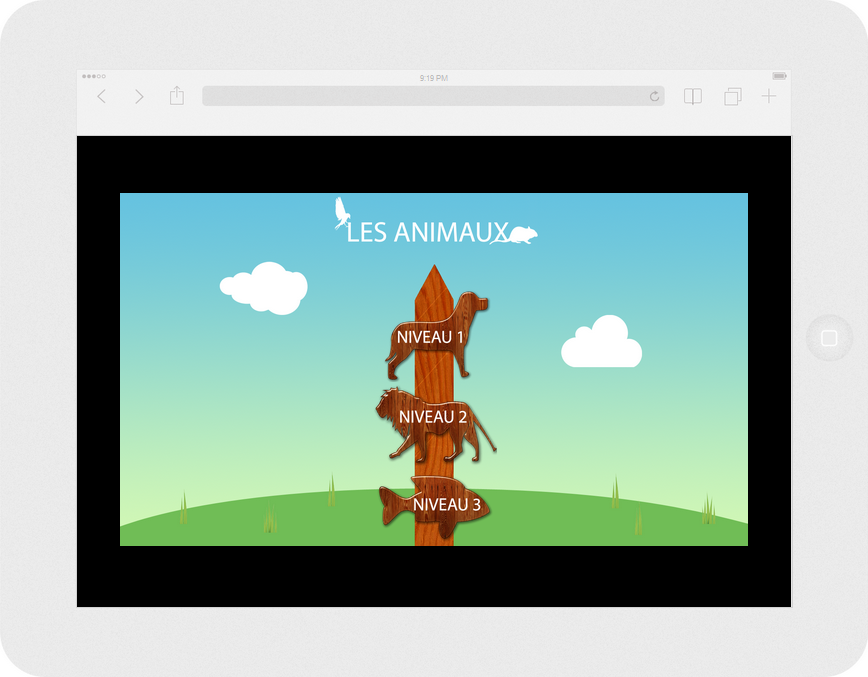
\includegraphics[width=0.8\textwidth]{tablette}\\
\vspace{3cm}
\textbf{Pr\'eambule}
\end{center}

\hspace*{0.6cm}Les jeux sont un bon moyen d'am\'eliorer les compétences logico-mathématiques et "corporelle-kinesthésiques" d'une personne. Mais ces effets sont décuplés sur les enfants. Poussés par leur curiosité et leur désir d'accomplissement, ils feront souvent tout ce qui est en leur pouvoir pour arriver à la fin d'un jeu. Ces sentiments, si bien maniés, peuvent permettre d'enseigner facilement les notions de base essentielles (à l'instar de la logique, de la rhétorique ou encore connaissances scientifiques en général) aux enfants, qu'ils soit handicapés ou non.
\vspace{0.5cm}\\
\hspace*{0.6cm}Notre jeu met le joueur devant un problème d'association logique entre plusieurs images. En début de partie, cinq images sont données au joueur et trois images en jaune sont quant à elles posées devant lui. Le joueur doit alors chercher le lien entre les images qu'il a et celles en jaune.

\newpage
\tableofcontents

\newpage
\section{Prérequis}
1. Un logiciel de décompression
\begin{itemize}
  \item Winrar
  \item Winzip (Installé de base avec Windows)
\end{itemize}
2. Un navigateur web 
\begin{itemize}
  \item Internet explorer (Version minimum 9)
  \item Google Chrome (Version minimum 44)
  \item Mozilla Firefox (Version minimum 40)
  \item Safari (Version minimum 5.1)
  \item Opera (Version minimum 12)
  \item iOS (Version minimum 6.1)
  \item Android (Version minimum 2.3)
\end{itemize}

\newpage
\section{Installation}
\subsection{Décompression}
\hspace*{0.6cm}Décompresser l'archive par un simple clique droit puis extraire ici comme le montre l'image ci-dessous :\\
(Une installation de Winrar sera peut-être nécessaire)
\vspace{0.5cm}\\
\fbox{
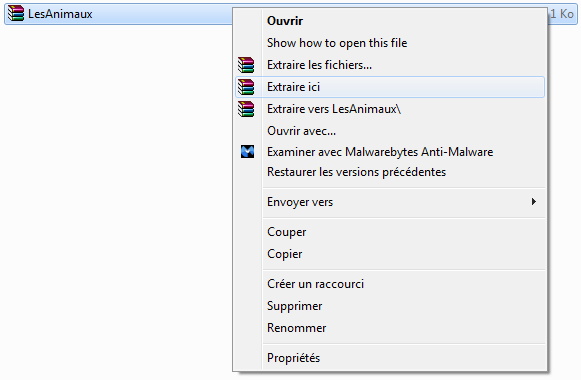
\includegraphics[width=1.0\textwidth]{winrar}\\
}
\subsection{Lancement}
Cliquer ensuite sur le dossier apparu puis sur le fichier nommé "index" ou "index.html" :
\vspace{0.5cm}\\
\fbox{

\includegraphics[width=1.0\textwidth]{index}\\
}
\subsection{Plein écran}
Il est possible de mettre le jeu en plein écran en appuyant sur F11 une fois le jeu arrivé sur l'écran d'accueil. 

\newpage
\section{Gameplay}

Le jeu est décomposé en deux parties. En haut (zone1 en rouge), vous trouverez les animaux que vous pouvez déplacer et en bas (zone 2 en violet) les zones o\`u vous pouvez les déplacer.
\vspace{0.5cm}
\begin{center}
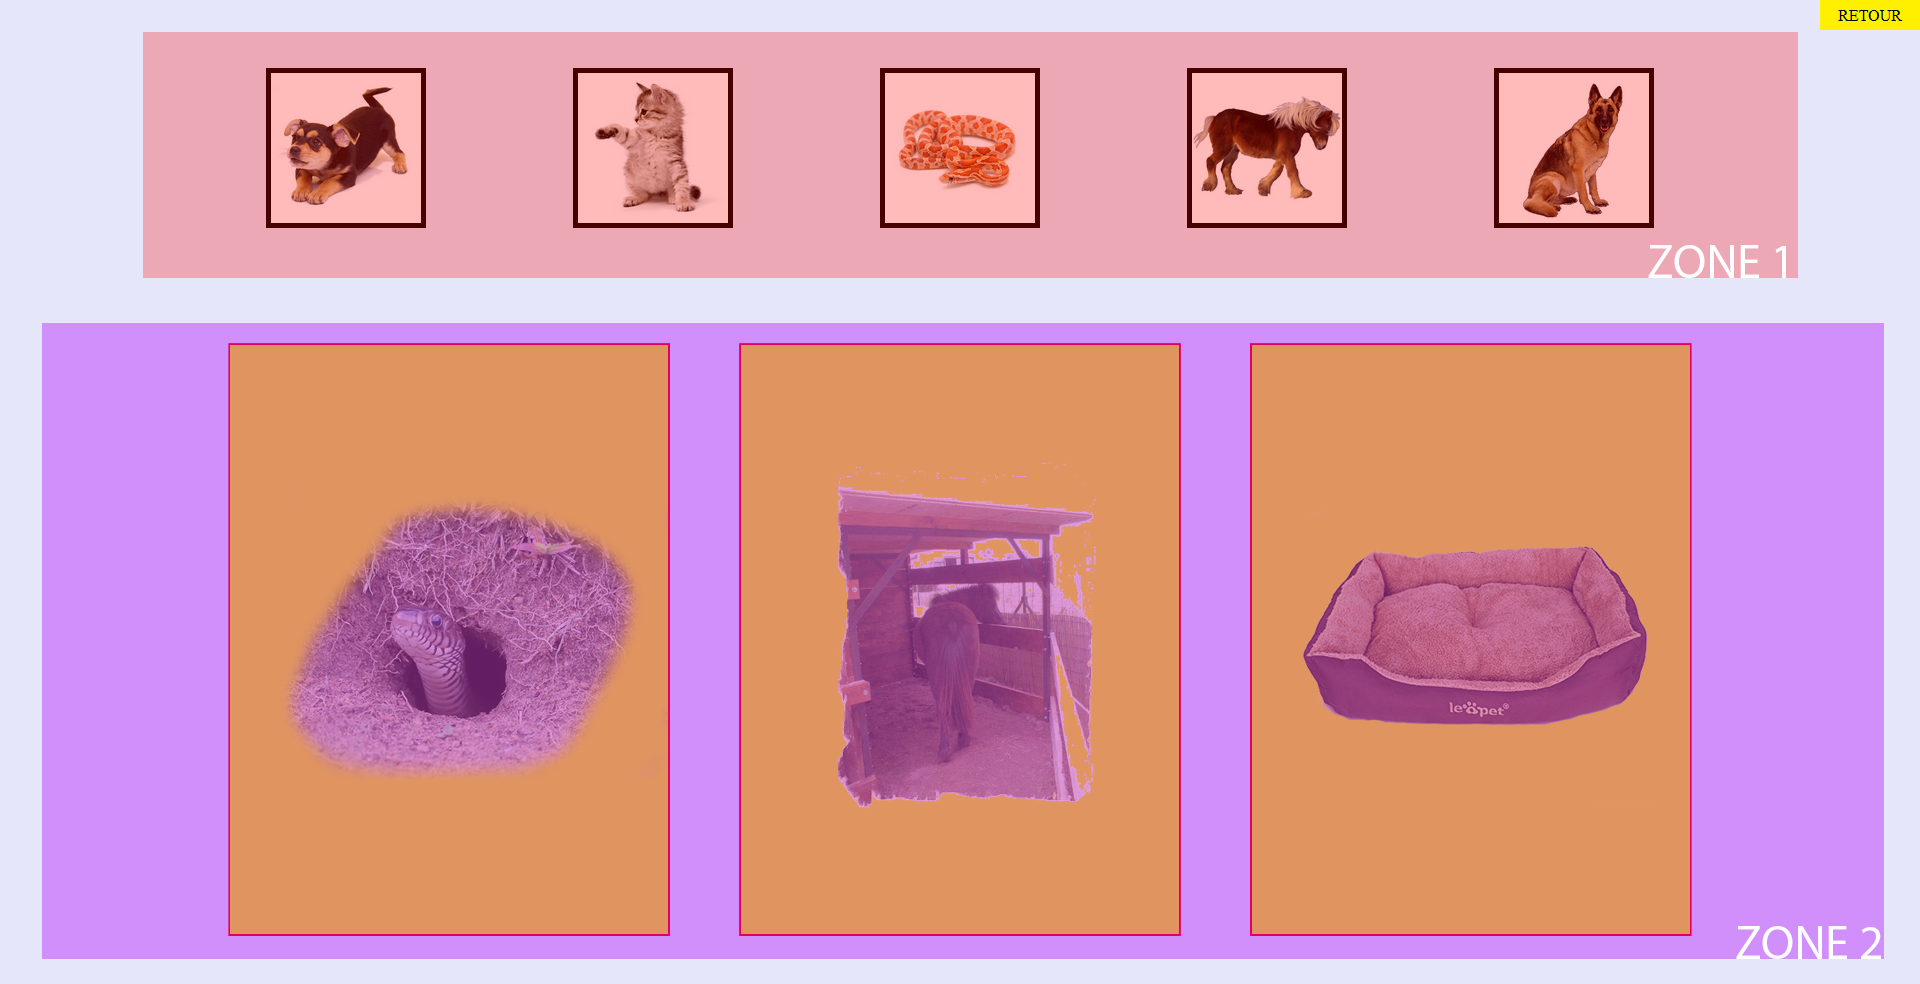
\includegraphics[width=0.75\textwidth]{zone}
\end{center}
\vspace{0.5cm}
Le but du jeu est de déplacer les animaux de la zone 1 vers la zone 2 en suivant une certaine logique. Reprenons notre exemple précédent et notons les animaux de la zone 1.\\
\vspace{0.5cm}
\begin{center}
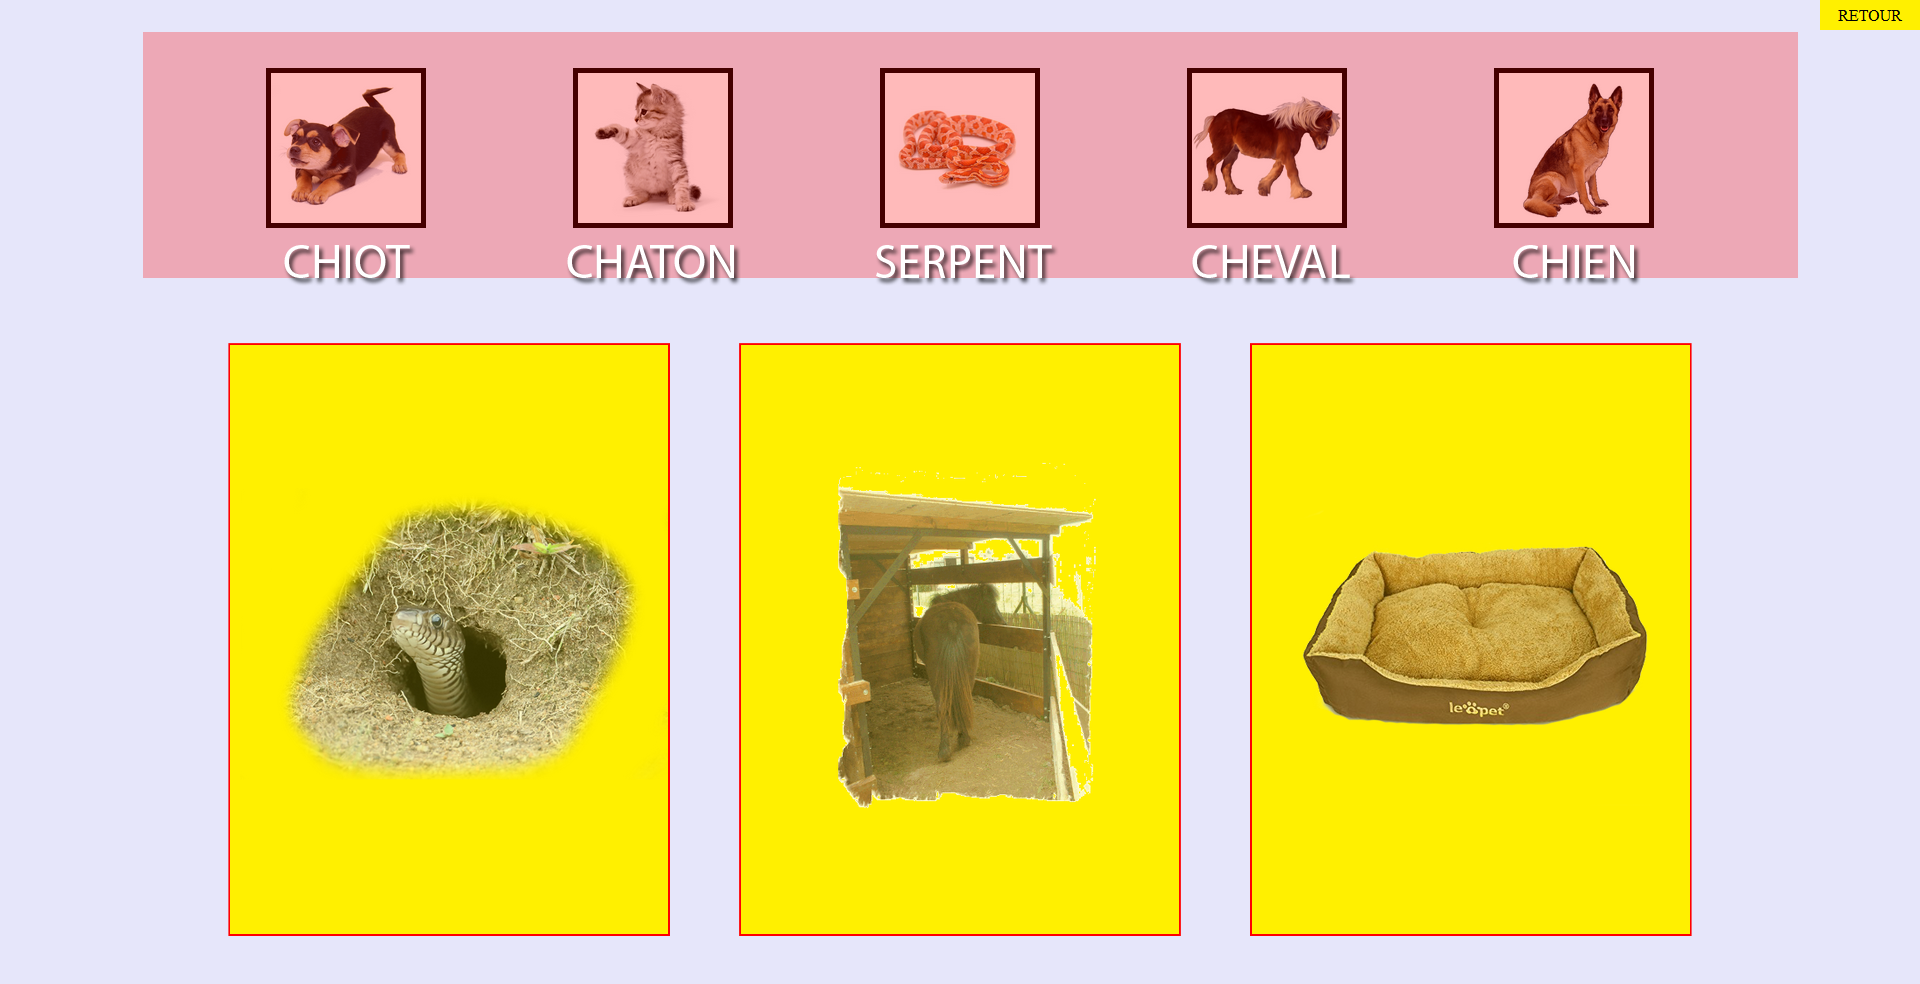
\includegraphics[width=0.75\textwidth]{zone1}
\end{center}
\vspace{0.5cm}
Prenons par exemple le cheval, nous allons cliquer dessus et maintenir notre clic tout en dépla\c{c}ant la souris.
\vspace{0.5cm}\\
\begin{center}
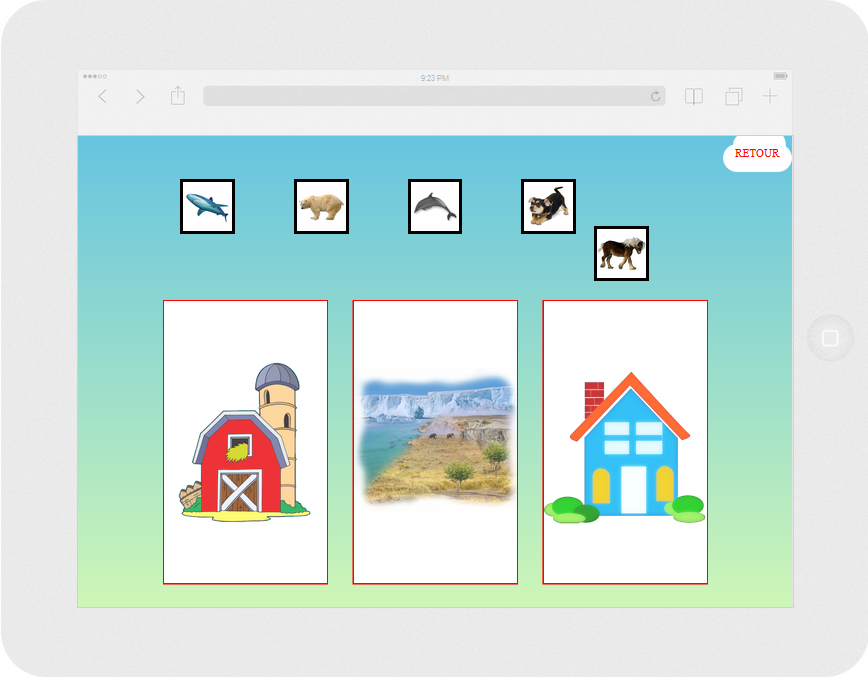
\includegraphics[width=0.75\textwidth]{zone2}
\end{center}
\vspace{0.5cm}
Si nous rel\^achons notre clic, l'image du cheval retournera à sa place automatiquement. Maintenant, regardons avec attention la zone 2 et décrivons là aussi les images. 
\vspace{0.5cm}\\
\begin{center}
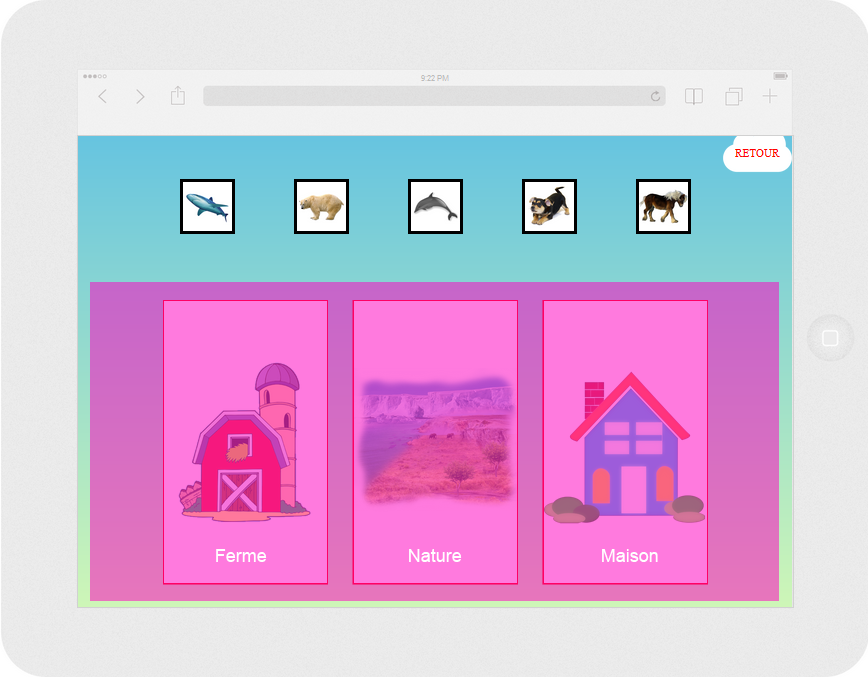
\includegraphics[width=0.75\textwidth]{zone3}
\end{center}
\vspace{0.5cm}
Reprenons maintenant notre cheval et dépla\c{c}ont le dans la zone qui lui correspond (la ferme). L'image se fixera alors à la zone et vous ne pourrez plus y toucher. Vous avez la bonne réponse !
\vspace{0.5cm}\\
\begin{center}
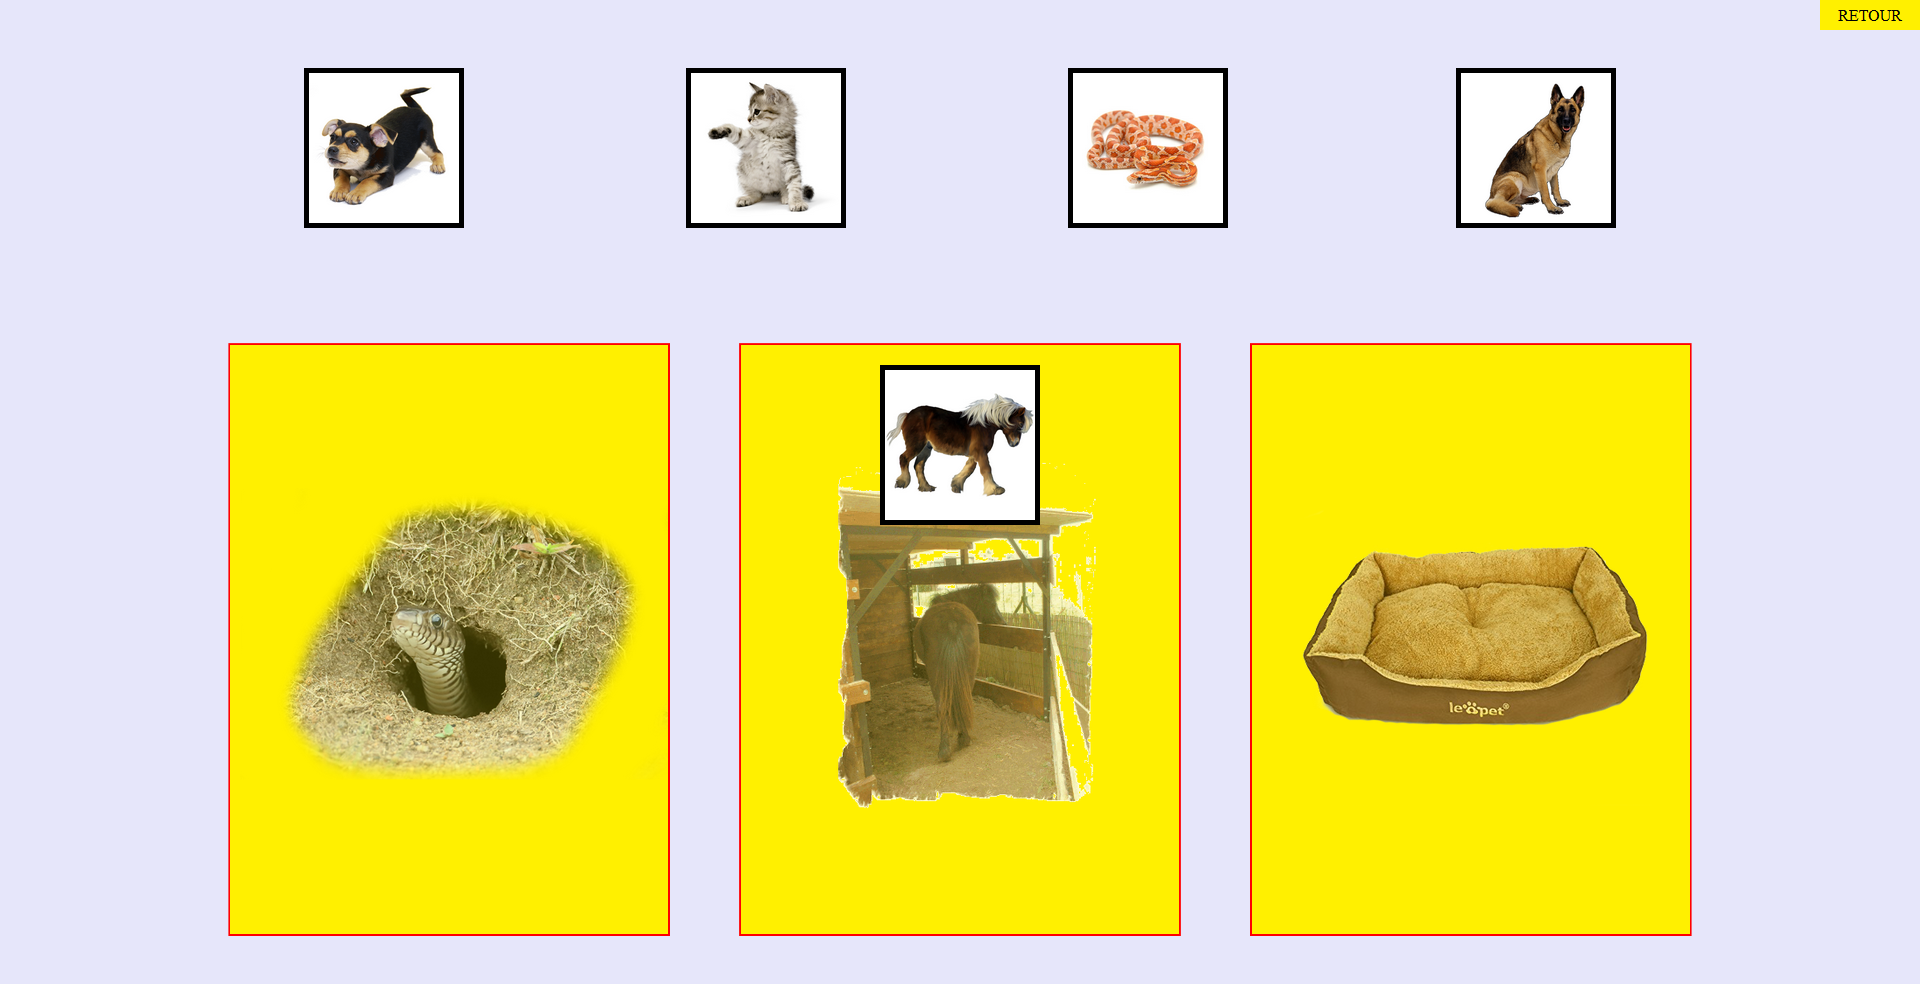
\includegraphics[width=0.75\textwidth]{zone4}
\end{center}
\vspace{0.5cm}
Maintenant effectuons cette même opération pour chaque image restante dans la zone 1. Allez, encore un petit effort, nous y sommes presque.
\vspace{0.5cm}\\
\begin{center}
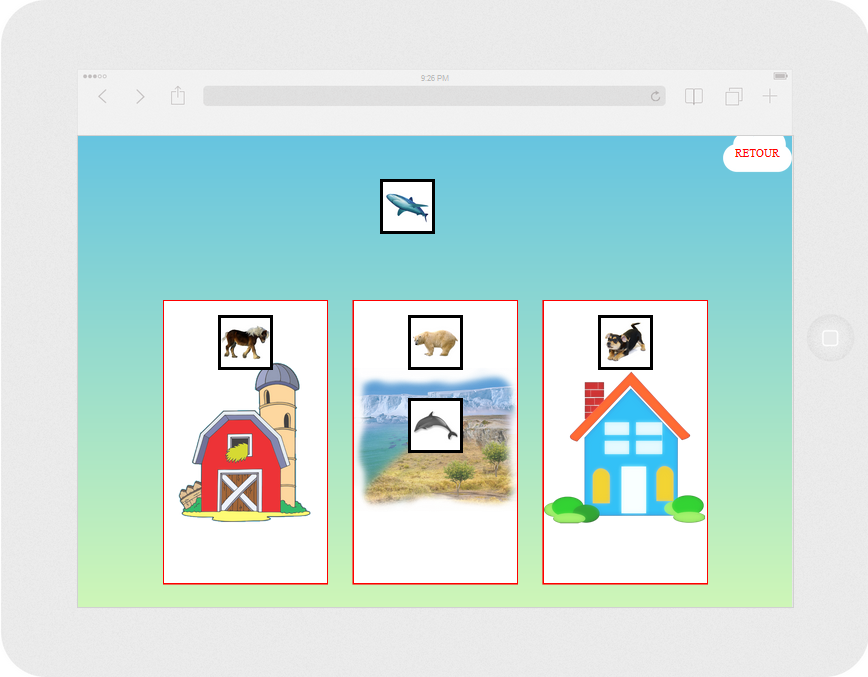
\includegraphics[width=0.75\textwidth]{zone5}
\end{center}
\vspace{0.5cm}
Si vous répondez correctement en pla\c{c}ant l'integralité des images, un message vous disant "Bravo" s'affiche alors pour vous féliciter.
\vspace{0.5cm}\\
\begin{center}
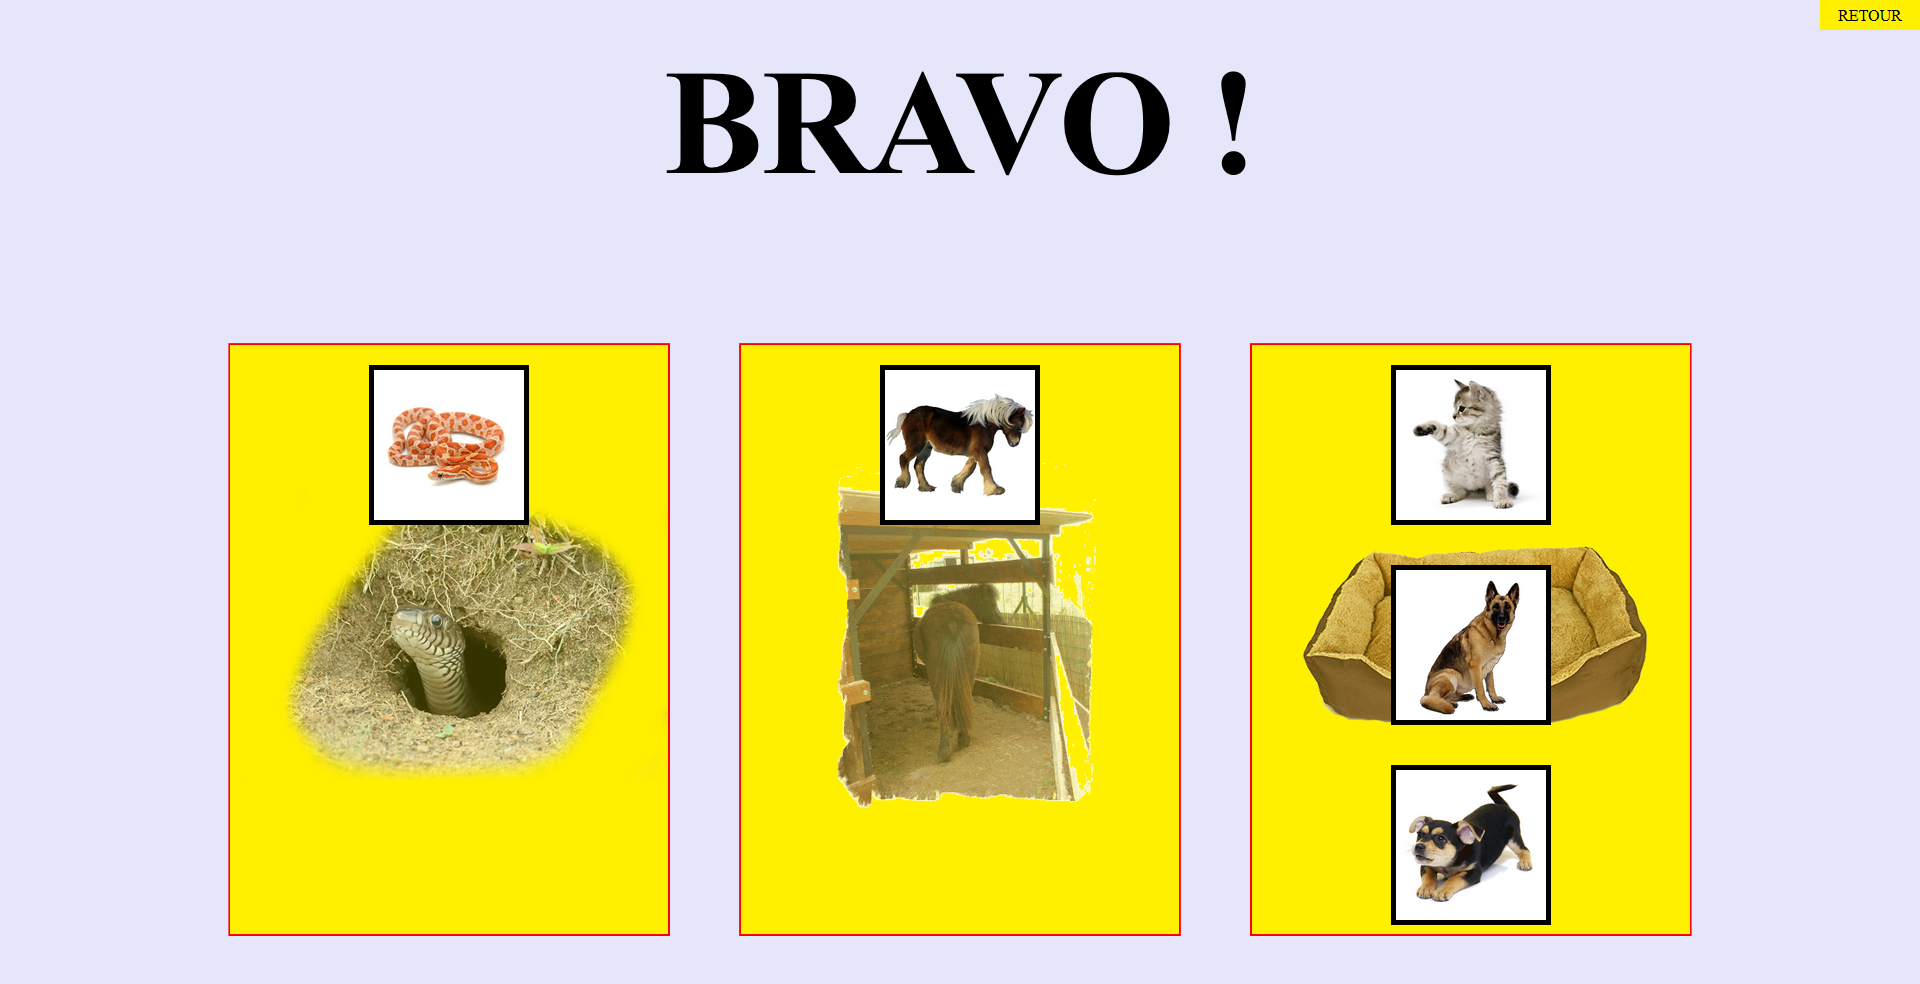
\includegraphics[width=0.75\textwidth]{zone6}
\end{center}
\vspace{0.5cm}
Puis une nouvelle partie commence avec de nouveaux éléments dans les deux zones.
\vspace{0.5cm}\\
\begin{center}
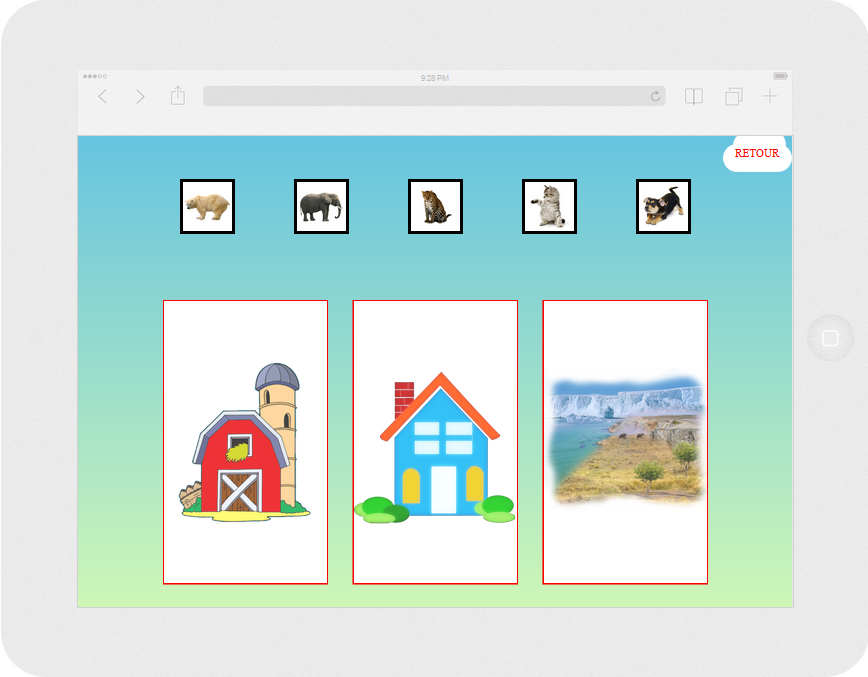
\includegraphics[width=0.75\textwidth]{zone7}
\end{center}
\vspace{0.5cm}

\newpage
\section{\'Evolutions}

Si quelqu'un reprenait le jeu et voudrait l'améliorer, il faudrait selon moi seulement ajouter du contenu ou encore simplement donner la possibilité aux joueurs de spécifier le nombre d'élément en bas et en haut. Une sorte de niveau de difficulté paramétrable dans les différents niveaux.

\newpage
\section{Outils nécessaires au développement}

\hspace*{0.6cm}Le jeu a été entièrement codé et réalisé en HTML5, CSS et JAVASCRIPT via la librairie JQUERY. Les fichiers du jeu sont lisibles et interprétés par tous les navigateurs existants en 2015.\\
\hspace*{0.6cm}Nous avons aussi utilisé LaTeX pour établir nos documents textuels, les différents navigateurs internet pour essayer le jeu ainsi que Photoshop pour la modification des images.\\
Pour partager le code efficacement, nous avons utilisé GIT.

\end{document}